\documentclass[a4paper, 11pt]{article}

% Nécessaire
\usepackage[utf8]{inputenc}
\usepackage[T1]{fontenc}
\usepackage{lmodern}

% Biblio
\usepackage{natbib}
\bibliographystyle{abbrvnat}
\usepackage{hypernat}
\bibpunct{\textcolor{blue}{[}}{\textcolor{blue}{]}}{}{a}{\textcolor{blue}{,}}{;}

\usepackage[french]{babel}
\usepackage{amsmath, amsthm}
\usepackage{amsfonts,amssymb}

% Marge
\usepackage{geometry}
\geometry{margin={2.2cm ,2cm}}

% Figures, graphiques
\usepackage{graphicx}
\usepackage{epsfig}
\usepackage{caption}

% Surlignage
\usepackage{alltt}

\usepackage{xcolor}
\usepackage{soul}
\usepackage{color}
\usepackage{colortbl}

% Indicatrice
\usepackage{dsfont}

\usepackage{multirow}
\usepackage{eurosym}
\usepackage{extarrows}
\usepackage[colorlinks=true, citecolor=blue, linkcolor=.]{hyperref}

% Graphique
\usepackage{tikz}


% Titre
\title{Estimation sur 100 jours}
\author{}
\date{}



\begin{document}
 \maketitle
 
On a prolongé l'estimation au-delà des 80 jours d'observations. Le nombre d'inflorescences fût mis à 1.

Résultats
\begin{figure}[ht]
\centering
 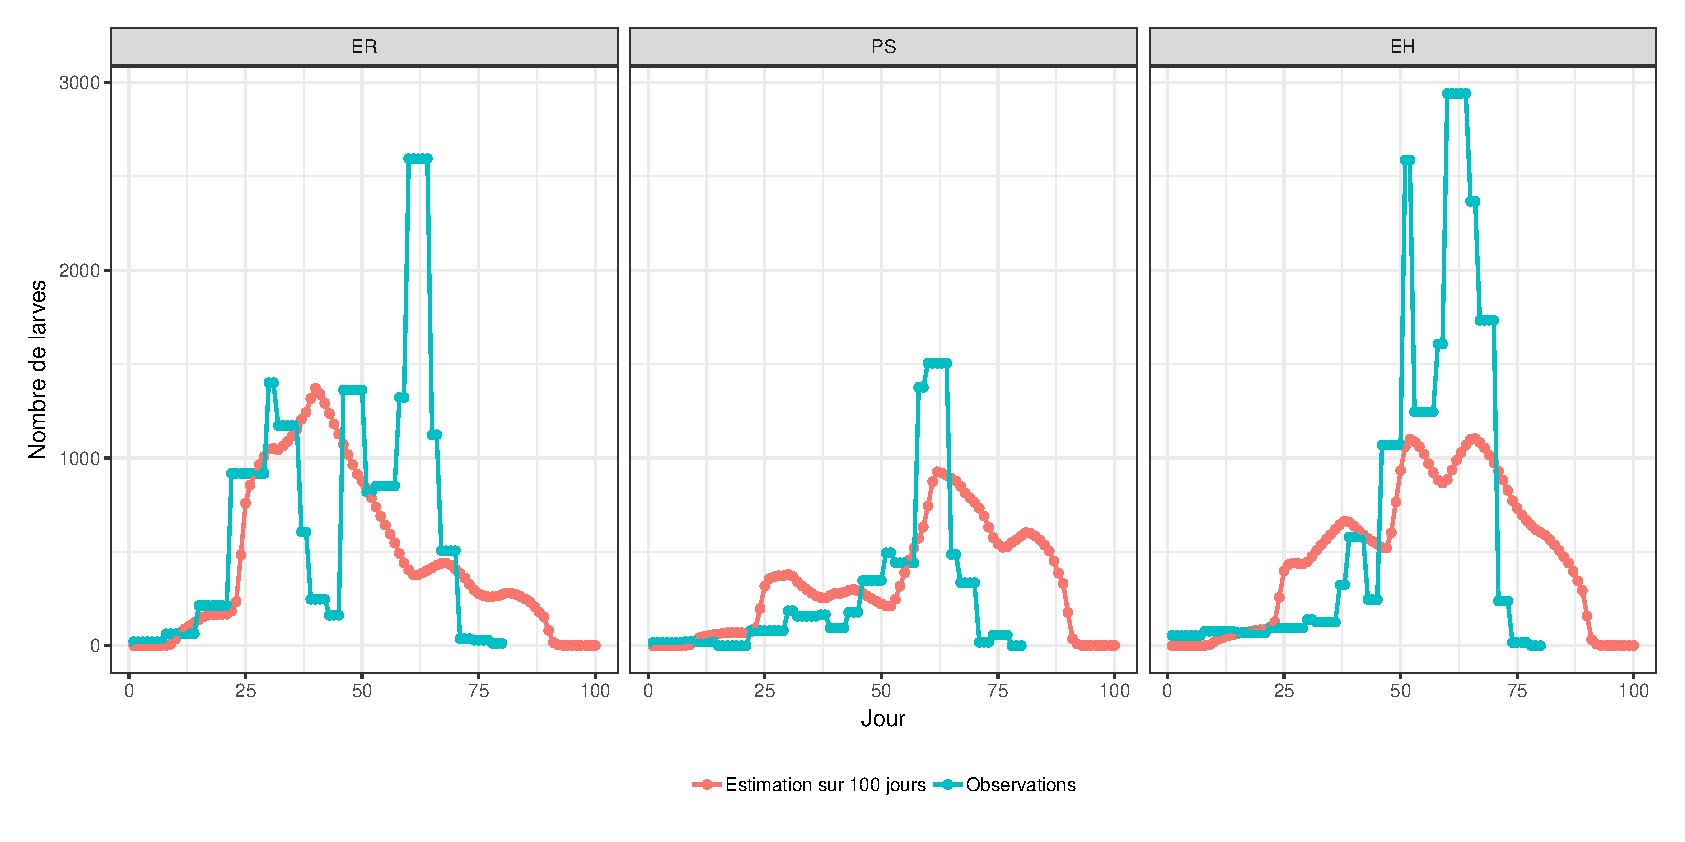
\epsfig{file = plots/centj.eps, scale = 0.59}
\end{figure}

La chute des larves à 0 n'intervient que 12 jours après la fin des inflorescences. Cela correspond à la durée de développement larvaire.

\end{document}

